\documentclass[11pt]{article}

% load some asm stuff -
\usepackage{amssymb}
\usepackage{amsmath}
\usepackage{amsthm}
%\usepackage{palatino,lettrine}
\usepackage{fancyhdr}
\usepackage{epsfig}
\usepackage[square,sort,comma,numbers]{natbib}
\usepackage{simplemargins}
\usepackage{setspace}
\usepackage{wrapfig}
\usepackage{hyperref}
%\usepackage{boiboites}
\usepackage[margin=0pt,font=small,labelfont=bf]{caption}
\newcommand{\boldindex}[1]{\textbf{\hyperpage{#1}}}
\usepackage{makeidx}\makeindex
\bibliographystyle{plos2015}


\usepackage{algpseudocode}
\usepackage{algorithm}

% Set the size
%\textwidth = 6.75 in
%\textheight = 9.75 in
%\oddsidemargin = 0.0 in
%\evensidemargin = 0.0 in
%\topmargin = 0.01 in
%\headheight = 0.0 in
%\headsep = 0.25 in
%\parskip = 0.15in
% \doublespace
\setallmargins{1in}

\newtheorem{example}{Example}[section]
\newtheorem{thm}{Theorem}[section]
\newtheorem{property}{Property}[section]

\theoremstyle{definition}
\newtheorem{defn}[thm]{Definition}

\makeatletter
% \renewcommand\subsection{\@startsection
% 	{subsection}{2}{0mm}
% 	{-0.05in}
% 	{0.1\baselineskip}
% 	{\normalfont\normalsize\bfseries}}
\renewcommand\subsubsection{\@startsection
	{subsubsection}{2}{0mm}
	{-0.05in}
	{-0.5\baselineskip}
	{\normalfont\normalsize\itshape\bfseries}}
\renewcommand\paragraph{\@startsection
	{paragraph}{2}{0mm}
	{-0.05in}
	{-0.5\baselineskip}
	{\normalfont\normalsize\itshape}}
\makeatother
\linespread{1.1}

\fancypagestyle{proposal}{\fancyhf{}%
	\fancyhead[RO,LE]{\thepage}%
	\fancyhead[LO,RE]{CHEME 5660 Pricing Treasury Securities}%
	\renewcommand\headrulewidth{1pt}}
\pagestyle{proposal}

\usepackage{mdframed}
\definecolor{lgray}{rgb}{0.92,0.92,0.92}
\definecolor{antiquewhite}{rgb}{0.98,0.92,0.84}
\definecolor{lightskyblue}{rgb}{0.93,0.95,0.99}

% defn environment
\mdfdefinestyle{theoremstyle}{% 
    linecolor=black,linewidth=1pt,% 
    frametitlerule=true,% 
    frametitlebackgroundcolor=lgray, 
    innertopmargin=\topskip,} 
\mdtheorem[style=theoremstyle]{definition}{Definition}

% concept environment
\mdfdefinestyle{conceptstyle}{% 
    linecolor=black,linewidth=1pt,% 
    frametitlerule=true,% 
    frametitlebackgroundcolor=lightskyblue, 
    innertopmargin=\topskip,} 
\mdtheorem[style=conceptstyle]{concept}{Concept}
\newcommand{\newterm}[1]{{\it #1}}

% Single space'd bib -
\setlength\bibsep{0pt}

\renewcommand{\rmdefault}{phv}\renewcommand{\sfdefault}{phv}
%\newboxedtheorem[boxcolor=black, background=gray!5,titlebackground=orange!20,titleboxcolor = black]{color_box_example}{Example}{test}

% Change the number format in the ref list -
\renewcommand{\bibnumfmt}[1]{#1.}

% Change Figure to Fig.
\renewcommand{\figurename}{Fig.}
\usepackage{enumitem}
\setlist{noitemsep} % or \setlist{noitemsep} to leave space around whole list

%Joycelyn Chan, Joshua Lequieu, Michael Paull, Chidanand Balaji, Ryan Tasseff
%Our derivation follows closely the earlier development of Fredrickson \citep{Fredrickson:1976fk}.

% Begin ...
\begin{document}

%\begin{titlepage}
{\par\centering\textbf{\Large Unit 1: Abstract Assets and the Pricing of Treasury Securities}}
\vspace{0.2in}
{\par \centering \large{Jeffrey D. Varner}}
\vspace{0.05in}
{\par \centering \large{Smith School of Chemical and Biomolecular Engineering}}
{\par \centering \large{Cornell University, Ithaca NY 14853}}
% \vspace{0.1in}
% {\par \centering \small{Copyright \copyright\ Jeffrey Varner 2018. All Rights Reserved.}}\\

%\end{titlepage}
\date{}
\thispagestyle{empty}

\setcounter{page}{1}

\tableofcontents
\clearpage
\listoffigures
\clearpage
\listofalgorithms
\clearpage

\section{Preliminaries}
We'll use concepts and approaches from finance, mathematics, statistics, and computer science throughout all the courses.
Let's begin this module by reviewing some of these concepts, particularly the idea of an abstract asset and the time value of money.
These two foundational concepts are essential for understanding the pricing of zero-coupon Treasury securities (and other financial instruments).
They also provide a useful framework for financial decision-making.

\subsection{Abstract Assets}
The traditional view of an \href{https://en.wikipedia.org/wiki/Asset}{asset} is perhaps a physical resource with economic value that an individual, corporation, or country owns or controls with the expectation that it will provide a future benefit.
For example, a car, house, or land are all assets.
However, in a more general sense, we can also think of an asset as a sequence of current and future cash flows demarcated in some currency, for example, Euros, Dollars, Yuan, or cryptocurrencies such as Bitcoin.
This more general notion of an asset, which we'll refer to as an \newterm{abstract asset}\index{Abstract asset}, is a useful mental model for thinking about the pricing of financial instruments, e.g., stocks, bonds, and derivatives, 
as well as the valuation of projects, other investments, and even traditional physical assets.
In this model, cash flows can be positive or negative, and assets can be tangible or intangible.
The challenge with this framework is that current and future cash flows are not directly comparable,
i.e., we cannot add or subtract a cash flow that occurs today from a cash flow that occurs at a different time in the future.
These cash flows can be thought of as being in different currencies, e.g., dollars versus euros, that must be exchanged. Thus, we formulate the equivalent of an exchange rate to compare cash from various periods.
This is the concept of the time value of money, discount factors, and discount rates, which we will discuss next.

\subsection{Time Value of Money}
At first glance, the idea that money has a time value seems counterintuitive. 
If I put a dollar in my pocket today, it is still a dollar tomorrow, next week, or next year. 
However, the value of a dollar today, e.g., the Utility it brings to you by purchasing a good or service, is not the same as the value of a dollar tomorrow.
The change in the value of money over time is called the time value of money (Concept \ref{concept:time-value-of-money}):
\begin{concept}[Time value of money]\label{concept:time-value-of-money}
	One dollar today is not worth the same as one dollar tomorrow. 
	The change in the value of money over time is called the \newterm{time value of money}\index{The time value of money}.
\end{concept}
The time value of money is an empirical observation that has been seen over hundreds of years. 
But why is this the case? Short answer: Money given to us today has a greater \href{https://en.wikipedia.org/wiki/Utility}{Utility} than the same amount tomorrow because we have an extra day to invest (or use) that money. Suppose a \emph{risk-free} investment is guaranteed to return an interest rate of $i>0$ per period.
If we invested $P$ dollars today in this risk-free investment, at the end of the investment period, e.g., a day, week, year, etc., 
we are \emph{guaranteed} to get $F$ dollars back (because the investment is risk-free):
\begin{equation*}
F = (1+i)\cdot{P}
\end{equation*}
where $F$ is the future value of the investment, $P$ is the present value of the investment, and $i$ is the interest rate per period.
Thus, if given a choice between $P$ dollars today or $P$ dollars one investment period in the future, 
a rational investor would always choose to take the $P$ dollars now. By taking $P$ dollars today, you could invest those $P$ dollars risk-free and get $F = (1+i)\cdot{P}$ back, where $F>P$. 
In this hypothetical world, the only case where it makes sense to take the future money is if $i\leq{0}$, i.e., $F\leq{P}$, which is forbidden by the condition $i>0$. 
This hypothetical scenario assumes that a risk-free investment exists that always returns an interest rate of $i>0$; 
does such an investment exist? 

\href{https://www.investopedia.com/terms/r/risk-freerate.asp}{Unfortunately, an actual risk-free investment is only a theoretical concept}. 
However, the risk-free rate of return $i$ is often approximated by the yield on US Treasury debt securities because the full faith and credit of the United States government backs US Treasury debt securities
and are considered one of the safest investments in the world. 
Thus, we can use the yield on US Treasury debt securities as a proxy for the risk-free rate of return $i$. 
This is the first reason why we are interested in these securities.

\subsection{Discrete exchange rate model}
Now that we have established money’s present value is higher than its future value, we need a way to compare cash from different periods. 
A useful mental model for the time value of money is to think of money from different periods 
as being in other currencies (e.g., dollars versus euros) that must be exchanged. 
Thus, we can formulate the equivalent of an exchange rate to compare money or cash flows from different periods. 
For example, suppose we have an active asset over multiple periods, e.g., a multi-period project or some other transaction that occurs over many periods. 
Further, suppose we have a cash flow $\dot{c}_{t}$ in period $t$ that we want to convert to a cash flow $\dot{c}_{0}$ in period zero, e.g., the future sale of shares of stock.
In this case, we develop a multi-period conversion that is easily constructed by sequentially applying many one-period calculations. To see this idea, let's start with period zero to period one:
\begin{equation}\label{eq:period-zero-to-one}
\dot{c}_{1} = \left(1+r_{10}\right)\cdot\dot{c}_{0}
\end{equation}
where $r_{10}$ is the exchange rate (what we'll later call the \texttt{short rate}) from period zero to period one, and $\dot{c}_{0}$ is the cash flow in period zero.
Then, period one to period two is given by:
\begin{equation}\label{eq:period-one-to-two}
\dot{c}_{2} = \left(1+r_{21}\right)\cdot\dot{c}_{1}
\end{equation}
where $r_{21}$ is the exchange rate from period one to period two, and $\dot{c}_{1}$ is the cash flow in period one. 
However, we can substitute $\dot{c}_{1}$ from Equation \ref{eq:period-zero-to-one} into Equation \ref{eq:period-one-to-two} to give:
\begin{equation}\label{eq:period-one-to-two-substituted}
\dot{c}_{2} = \Bigl[\left(1+r_{21}\right)\left(1+r_{10}\right)\Bigr]\cdot\dot{c}_{0}
\end{equation}
If we do this computation between 2 and 3, and then 3 to 4, etc, we develop a relationship between the initial value of cash flow 
$\dot{c}_{0}$ and future $\dot{c}_{t}$ cash flow values (Defn. \ref{defn:multiple-period-discrete-conversion}):

\begin{definition}[Multiple period-dependent discrete discount]\label{defn:multiple-period-discrete-conversion}
Assume discrete compounding and one compounding event per period. Let $\dot{c}_{j}$ denote cash flow events in period(s) $j = 0,1,2,\dots$ 
and $r_{j+1,j}\geq{0}$ denote the discount rate between periods $j\rightarrow{(j+1)}$.
Then, by induction, cash flow events are related by the expression
\begin{equation*}
\dot{c}_{k} = \left[\prod_{j=0}^{k-1}\left(1+r_{j+1,j}\right)\right]\cdot\dot{c}_{0}\qquad{k=0,1,2,\dots}
\end{equation*}
The product term is the \textit{multi-period discrete discount factor} or $\mathcal{D}_{k,0}(r)\geq{1}$.
\begin{itemize}[leftmargin=*]
	\item{For $k=0$: The present and future value are equal which means that $\mathcal{D}_{0,0}(r) = 1$.}
	\item{For $k\geq{1}$: The discount factor $\mathcal{D}_{k,0}(r)>{1}$ for positive discount rates $r_{j+1,j}>0$.}
\end{itemize}

% Let $\dot{c}_0$ be the present cash flow, and $\dot{c}_t$ be the future cash flow in period $t$. 
% Further, let $r_{j+1,j}$ represent the discount rate between discrete periods $j$ and $j+1$. Then: 
% \begin{equation}
% \dot{c}_{t} = \left[\prod_{j=0}^{t-1}\left(1+r_{j+1,j}\right)\right]\cdot\dot{c}_{0}\qquad{t=1,2,\dots,T}
% \end{equation}
% The term in the brackets is the \textit{multi-period discrete discount factor}, which we represent as the function $\mathcal{D}_{t,0}(r)$.
\end{definition}

Of course, an obvious challenge with this approach is that we need to know the discount rate(s) $r_{j+1,j}$ between every period $j$ and $j+1$.
In practice, this is not possible. However, suppose we  approximated the discount rate(s) $r_{j+1,j}$ with an effective rate $\bar{r}$ 
that was constant over the lifetime of the project or investment such that:
\begin{equation}\label{eq:effective-rate}
\left(1+\bar{r}\right)^{t} = \prod_{j=0}^{t-1}\left(1+r_{j+1,j}\right)
\end{equation}
For the special case when the discount rate is constant $\bar{r}\equiv{r_{j+1,j}},\forall{j}$, the discrete multistep discount factor
can be rewritten as:
\begin{equation}\label{eq:multi-period-discrete-discount-factor}
\mathcal{D}_{k,0}(\bar{r}) = \left(1+\bar{r}\right)^k
\end{equation}
where $\bar{r}$ is the effective discount rate. Finally, imagine the we have $n$ compounding periods per year, 
and the effective discount rate $\bar{r}$ is an annualized rate (typically the case). 
Then, we can rewrite the effective discount rate as:
\begin{equation}\label{eq:effective-rate-compounded}
\mathcal{D}_{t,0}(\bar{r}) = \left(1+\frac{\bar{r}}{n}\right)^{n\cdot{t}}
\end{equation}
where $\bar{r}$ is the discount rate, and $n$ is the number of discounting events per period
(Defn. \ref{defn:multiple-effective-period-discrete-conversion}).
\begin{definition}[Multiple period effective discrete discount]\label{defn:multiple-effective-period-discrete-conversion}
	Let $\dot{c}_0$ be the present cash flow, and $\dot{c}_t$ be the future cash flow in period $t$. 
	Further, let $\bar{r}$ represent the (constant) effective discount rate, and $n$ is the number of discounting events per period. 
	Then:
	\begin{equation}
	\dot{c}_{t} = \left[\left(1+\frac{\bar{r}}{n}\right)^{n\cdot{t}}\right]\cdot\dot{c}_{0}\qquad{t=1,2,\dots,T}
	\end{equation}
	The term in the brackets is the \textit{multi-period effective discrete discount factor}, which we represent as the function $\mathcal{D}_{t,0}(\bar{r})$.
\end{definition}

\subsection{Continuous exchange rate model}
In the exchange rate model, we converted cash flows from the future to the present (and vice-versa) using a period-dependent discount rate $r_{t+1,t}$, 
or an effective discount rate $\bar{r}$, and a discount factor $\mathcal{D}_{t,0}(r)$. These acted like exchange rates between different currencies.
However, this approach is often seen as confusing. For example, it is unclear what discount rate to use, what a discount factor means practically, etc.
Toward this challenge, let's introduce a different perspective on discounting and the discount rate.
Suppose we think of the discount rate $r_{t+1,t}$  (or $\bar{r}$) as the minimum 
\newterm{rate of return}\index{rate of return} that a decision-maker 
would accept for a project or investment. In this context, discount rates are like interest rates we can earn on an investment.
Let's continue with this idea and introduce the concept of interest and interest rates.

There are two types of interest: simple and compound. The distinction between simple and compound interest is crucial in finance and investing.
These concepts significantly impact investment growth and borrowing costs, making them fundamental to consider when making financial decisions. 
Simple interest is paid only on the initial principle. 
For example, if the amount $A(0)$ is invested in an account at $t=0$ which pays a simple interest rate of $r$ per period, 
then after $k$ periods the account will hold amount $A(k)$ (assuming no withdrawals, etc):
\begin{equation}\label{eq:simple-interest}
A(k) = A(0)\cdot\left(1+rk\right)
\end{equation}
On the other hand, compound interest considers both the principal and the interest accumulated over time. 
For example, if amount $A(0)$ is invested in an account at $t=0$ which pays a compound interest rate $r$ per period, 
then after $k$ periods the account will hold amount $A(k)$ (assuming no withdrawals, etc):
\begin{equation}\label{eq:compound-interest}
A(k) = A(0)\cdot\left(1+r\right)^k
\end{equation}
If there are multiple compounding periods per year, then the interest rate $r$ is divided by the number of compounding periods per year $n$
and we arrive at the following expression for compound interest:
\begin{equation}\label{eq:compound-interest-multiple}
A(k) = A(0)\cdot\left(1+\frac{r}{n}\right)^{k\cdot{n}}
\end{equation}
Compound interest is more advantageous to the investor than simple interest. 
Furthermore, Eqn. \eqref{eq:compound-interest-multiple} is equivalent to Defn. \ref{defn:multiple-effective-period-discrete-conversion}
when the interest rate $r$ is the effective discount rate $\bar{r}$, and the number of compounding periods per year $n$ is the number of discounting events per period.
Finally, consider the case when the number of compounding periods per year $n\rightarrow\infty$, i.e., we have continuous compounding (Defn. \ref{defn:continuous-compounding}):
\begin{definition}[Continuous compounding]\label{defn:continuous-compounding}
% Let there be n-compounding periods per period, e.g., year, and an annualized interest rate of $r$.  
% Then an initial investment $A(0)$ will be worth:
% \begin{equation}\label{eqn-compound-interest-model-discrete}
% A(m) = A(0)\cdot\left(1+r/n\right)^{mn}
% \end{equation}
% after m-periods, e.g., m-years. As the number of compounding periods $n\rightarrow\infty$, 
% the investment $A(m)$ approaches the continuous compounding limit:
% \begin{equation}\label{eqn-compound-interest-model-cont}    
% \lim_{n\rightarrow\infty}A(m) = A(0)\cdot\exp\left(rm\right)
% \end{equation}
% The quantity $\exp\left(rm\right)$ is the \textit{continuous compounding (discount) factor}, 
% which we also represent (with a slight abuse of notation) as $\mathcal{D}_{m,0}(r)$.
Suppose we have a constant annualized discount rate $\bar{r}\geq{0}$ and $n$ compounding events yearly. Then, the discrete 
multistep discount factor for $k\geq{0}$ periods is given by:
\begin{equation*}
\mathcal{D}_{k,0}(\bar{r}) = (1+\bar{r}/n)^{k\cdot{n}}
\end{equation*}
However, suppose $n\rightarrow\infty$, i.e., we move to continuous compounding (compounding events at every instant).
Then, the discount factor $\mathcal{D}_{k,0}(\bar{r})$ becomes the \textit{continuous discount factor}:
\begin{equation*}
    \lim\limits_{n\rightarrow\infty}\mathcal{D}_{k,0}(\bar{r}) = \exp\left(r\cdot{k}\right)
\end{equation*}
\begin{itemize}[leftmargin=*]
\item{For $k=0$: The continuous discount factor, consistent with its discrete analog, is given by $\mathcal{D}_{0,0}(\bar{r}) = 1$.}
\item{For $k>0$: The continuous discount factor, consistent with its discrete analog, is given by $\mathcal{D}_{k,0}(\bar{r}) > 1$.}
\end{itemize}
\end{definition}
Continuous discount factors are used for equity and derivatives, while discrete discounting is used for Treasury securities.

\subsection{Net Present Value (NPV)}
Now that we have tools to account for the time value of money, we can return to the question of how to value an asset. 
The most intuitive approach is to compute the net cash flow over every period. Imagine at node $t=k$ we have $\mathcal{S}^{t=k}$ cash streams,
denoted as $\dot{c}_{s}$, entering (or exiting) the asset node. 
Then, the net cash flow at node $t=k$ is given by:
\begin{equation}\label{eq:net-cash-flow}
\bar{c}_{k} = \sum_{s\in\mathcal{S}^{t=k}}\nu_{s}\dot{c}_{s}
\end{equation}
where $\nu_{s}$ is a direction parameter; $\nu_{s}=+1$ if stream $s$ enters node $t=k$, $\nu_{s}=-1$ if stream $s$ exists node $t=k$. 
Finally, we sum all the current and future cash flows, converted to a shared basis, such as current dollars. 
This sum is called the Net Present Value (NPV) (Defn. \ref{defn:net-present-value}): 
\begin{definition}[Net Present Value (NPV)]\label{defn:net-present-value}
The Net Present Value (\texttt{NPV}) of an abstract asset is the sum of current and future discounted \textit{net cash flows} over a time horizon $T$, 
assuming a constant discount rate $\bar{r}$:
\begin{equation}    
\text{NPV}(T, \bar{r}) = \sum_{i=0}^{T}{\mathcal{D}_{i,0}^{-1}}(\bar{r})\cdot\bar{c}_{i} = \left<\mathcal{D}^{-1}(\bar{r}),\,\bar{c}\right>
\end{equation}
where the $\bar{c}_{i}$ denotes the \textit{net cash flow} in period $i$, 
$\mathcal{D}_{i,0}(\bar{r})$ is the multistep discount factor (either discrete or continuous) between periods $0\rightarrow{i}$, and
$\left<\cdot,\cdot\right>$ denotes the scalar (dot) product.
The \texttt{NPV} does not require that the discount rate be constant over the lifetime of the project or investment, 
but this is often assumed.

% Let $\bar{c}_{t}$ be the net cash flow in period $t$. 
% Then, the net present value (NPV) is the sum of current and future discounted cash flows:
% \begin{equation}    
% \text{NPV}(T,r) = \sum_{i=0}^{T}{\mathcal{D}_{i,0}^{-1}}(r)\cdot\bar{c}_{i}\qquad{T,r\geq{0}}
% \end{equation}
% where the term \texttt{T} is the number of time periods 
% (lifetime of the project or investment), and $\mathcal{D}_{i,0}(r)$ is the multistep discount factor with discount rate(s) \texttt{r}
% between period $i$ and period $0$.
% \begin{itemize}[leftmargin=*]
% \item{The discount factor $\mathcal{D}_{i,0}(r)$ can be either a discrete or a continuous discounting model.}
% \item{The NPV does not require that the discount rate is constant over the lifetime of the project or investment, but this is often assumed.}
% \item{The discount  $\mathcal{D}_{0,0}(r) = 1$ for all values of $r$.}
% \end{itemize}
\end{definition}
The net present value (NPV) is a helpful metric for financial decision-making.
In this context, the NPV has the following interpretations:
\begin{itemize}[leftmargin=*]
	\item{\texttt{NPV}$\,>\,0$: The abstract asset will \textbf{outperform} an alternative risk-free investment growing at the risk-free discount rate $\bar{r}$.}
	\item{\texttt{NPV}$\,=\,0$: The abstract asset will perform \textbf{the same as} an alternative risk-free investment growing at the risk-free discount rate $\bar{r}$.}
	\item{\texttt{NPV}$\,<\,0$: The abstract asset will \textbf{underperform} an alternative risk-free investment growing at the risk-free discount rate $\bar{r}$.}
\end{itemize}

% \begin{itemize}[leftmargin=*]
% \item{$\textbf{NPV}<0$:~}{A negative NPV indicates the proposed project will generate less income than a hypothetical alternative investment, e.g., a risk-free investment at the same discount rate and time-to-maturity as the project.}
% \item{$\textbf{NPV}=0$:~}{A zero NPV indicates the proposed project will generate the same income as a hypothetical alternative investment, e.g., a zero-coupon bond at the same discount rate and time-to-maturity as the project. }
% \item{$\textbf{NPV}>0$:~}{A positive NPV indicates the proposed project will generate more income than a hypothetical alternative investment, e.g., a zero-coupon bond at the same discount rate and time-to-maturity as the project.}
% \end{itemize}
The connection of the net present value (NPV) to the time value of money is clear.
However, the connection of the NPV with a zero-coupon bond is not. 
As we will see, the NPV of a project or investment with a zero NPV is equivalent to the price of a zero-coupon bond with the same time-to-maturity 
and discount rate. Thus, a rational investor would be indifferent between investing in an NPV = 0 project or investing in a zero-coupon bond.

\subsection{Internal Rate of Return (IRR)}
The NPV decision rule above relies on computing the sum of discounted future cash flows. 
However, in these calculations, what discount rate should we use? This question is difficult; the correct discount rate varies between applications and industries.  
The special discount rate where the net present value is zero is called the Internal Rate of Return (IRR) (Defn. \ref{defn:internal-rate-of-return}):

\begin{definition}[Internal Rate of Return (IRR)]\label{defn:internal-rate-of-return}
The Internal Rate of Return (\texttt{IRR}) is the effective (constant) discount rate $\bar{r}^{\star}\geq{0}$
that makes the net present value of an abstract asset equal to zero over a $T$-period time horizon:
\begin{equation}
\sum_{i=0}^{T}{\mathcal{D}_{i,0}^{-1}}(\bar{r}^{\star})\cdot\bar{c}_{i} = \left<\mathcal{D}^{-1}(\bar{r}^{\star}),\,\bar{c}\right> = 0
\end{equation}
where the $\bar{c}_{i}$ denotes the \textit{net cash flow} in period $i$, 
$\mathcal{D}_{i,0}(\bar{r})$ is the multistep discount factor (either discrete or continuous) between periods $0\rightarrow{i}$, and
$\left<\cdot,\cdot\right>$ denotes the scalar (dot) product.

% Assume the discount rate is constant between periods. Then, the internal rate of return (IRR) is the discount rate that makes the net present value equal to zero:
% \begin{equation}\label{eq:internal-rate-of-return}
% \sum_{t=0}^{T}{\mathcal{D}_{t,0}^{-1}}\cdot\bar{c}_{t} = 0
% \end{equation}
% The discount factor $\mathcal{D}_{t,0}$ can be modeled as either a discrete or a continuous discount factor. 
\end{definition}
Thus, the IRR is a decision boundary of sorts; the IRR is the discount rate at which the project manager or investor is indifferent to the project.
Discount rates greater than the IRR favor the alternative investment, while discount rates less than the IRR
favor the project.

\subsection{Summary}
In this section, we introduced the concept of an abstract asset, the time value of money, different discounting models, the net present value (NPV), and the internal rate of return (IRR).
We'll use these ideas throughout the course. However, in this unit, we'll use these concepts to develop a framework for pricing zero-coupon and multiple-coupon Treasury securities 
and to understand the risks associated with these securities.

\clearpage

\section{United States Treasury Securities}
\href{https://www.investor.gov/introduction-investing/investing-basics/glossary/treasury-securities}{United States Marketable Treasury Securities}, 
are issued by the U.S. Department of the Treasury to fund its operations and meet financial obligations. 
These debt securities are structured loan agreements between a borrower, i.e., the U.S. government, and a lender (you) 
that allows the government to fund its operations and obligations (Fig. \ref{fig:govt-debt-schematic}).
The debt holder and the U.S. Treasury have a marketable repayment agreement, which can be held by the lender (you) until the completion of the contract or resold on a secondary market. Although there are various types of U.S. government debt securities, they all share a few common characteristics. 
First, U.S. Treasury debt securities have a predetermined term length; thus, the contract duration between the borrower and lender is fixed.
Second, U.S. Treasury debt securities have a par value, representing the instrument's face value, a price (which may differ from the par value), and an interest rate paid to the lender. Next, some U.S. Treasury debt securities have interest payments commonly called coupons. These payments give the lender fixed cashflows on a predetermined schedule throughout the debt instrument's term. Finally, income from interest on U.S. Treasury debt securities is free of state and local income taxes but subject to federal income taxes.
You can purchase U.S. Treasury debt directly from the \href{https://www.treasurydirect.gov/indiv/products/prod_tbonds_glance.htm}{United States Treasury via TreasuryDirect} 
or through a bank or broker to lend money to the U.S. government.

\begin{figure}[h]
    \centering
    \includegraphics[width=0.85\textwidth]{./figs/Fig-Govt-Debt-Schematic.pdf}
    \caption{Schematic of U.S. Government Debt Securities. You lend money to the United States Treasury by purchasing a treasury security.
	The Treasury pays you back in different fixed ways, depending upon security.}\label{fig:govt-debt-schematic}
\end{figure}

\subsection{Risks of U.S. Treasury Securities}
While United States Treasury securities are considered to be risk-free, they are not without risk. The most obvious risk is the risk of default, i.e., the United States government could default on its obligations and not repay the debt holders (you).
This risk is considered very low, and the United States government has never, at least in recent memory, defaulted on its debt obligations (in the absence of technical issues). Other risks are associated with Treasury securities, including inflation and liquidity risks.
However, interest rate risk is the most significant non-default risk associated with Treasury securities.
The price of coupon-bearing Treasury securities is a function of the face (par) value of the security, the coupon rate, the yield (discount rate), and the number of coupon payments per year.
Thus, as these parameters change, e.g., the yield (discount rate), you would expect the price of the Treasury security to change (Concept \ref{concept:malkiel-theorems}):

\begin{concept}[Malkiel's Theorems]\label{concept:malkiel-theorems}
	Malkiel explored the question of bond pricing and proposed five theorems that relate the price of a coupon-bearing Treasury security to 
	changes in these parameters \citep{Malkiel-Bonds-1962}:
\begin{itemize}[leftmargin=*]
\item{\textbf{Theorem 1}: Bond prices move inversely to bond yields.}
\item{\textbf{Theorem 2}: For a given change in yield from the nominal yield, changes in bond prices are greater the longer the term to maturity. }
\item{\textbf{Theorem 3}: The percentage price changes described in Theorem 2 increase at a diminishing rate as N increases. }
\item{\textbf{Theorem 4}: Price movements resulting from equal absolute increases and decreases in yield are asymmetric; i.e., decreasing yields raise bond prices more than the same increase in yields lowers prices. }
\item{\textbf{Theorem 5}: The higher the coupon carried by the bond, the smaller the percentage price fluctuation for a given change in yield, except for one-year securities.}
\end{itemize}
\vspace{0.01in}
\noindent{\textit{Notation}}: when Malkiel refers to the yield, he is referring to the effective annual discount rate, $\bar{r}$. The coupon rate $\bar{c}$ in our bond (note) pricing model is the interest rate.
\end{concept}


\subsection{Zero-Coupon Treasury Bills}\label{sec:treasury-bills}
Let's focus on our first example of a U.S. Treasury security, the \href{https://treasurydirect.gov/marketable-securities/treasury-bills/}{Treasury Bill}.
\href{https://treasurydirect.gov/marketable-securities/treasury-bills/}{United States Treasury Bills}, \texttt{T-bills} or just \texttt{Zeros} are Treasury debt instruments with short-term maturity periods 
of T = 4, 8, 13, 26, and 52 weeks and zero coupon payments, i.e., no separate semiannual interest payments to the lender (you).
Perfectly priced T-bills are sold at a discount to their face value, and the difference between the purchase price and the face value is the return to the lender (you).
Treasury bills have a Net Present Value (NPV) of zero, i.e., the price of the T-bill is equal to its face value at maturity, escalated by the risk-free for the duration of the T-bill.

\subsubsection{Pricing of zero-coupon T-bills.}
In the context of the abstract asset framework, T-bills have two cashflow events, namely when the lender (you) buys the T-bill at auction 
and when the borrower (United States Treasury) pays the lender (you) the face (par) value of the T-bill at maturity (Fig. \ref{fig:t-bill-schematic}).
\begin{figure}[h]
    \centering
    \includegraphics[width=0.85\textwidth]{./figs/Fig-Bill-Asset-Timeline-Schematic.pdf}
    \caption{Asbtract asset schematic of a zero-coupon Treasury bill written from the perspective of the bill holder. The lender (you) gives the United States Treasury 
    the price $V_{B}$ of the T-bill at auction at $ t = 0$. In return, the Treasury pays the bill holder (you) the par value of the T-bill $V_{P}$ at maturity $t>0$. 
	For Treasury Biils, there are both cashflow events (solid arrows) and non-cashflow compounding events (dashed arrows).}\label{fig:t-bill-schematic}
\end{figure}
The price of a zero-coupon Treasury bill $V_{B}$ with an effective (constant) interest (discount) rate of $\bar{r}$ and a maturity of \texttt{T}-years at auction 
is the discounted face (par) value $V_{P}$ such that the net present value (NPV) of the bill is zero:
\begin{equation}    
\text{NPV}(T,\bar{r}) = -V_{B} + \mathcal{D}_{T,0}^{-1}(\bar{r})\cdot{V_{P}} = 0
\end{equation}
or equivalently:
\begin{equation}\label{eq:zero-coupon-treasury-bill-price}
    V_{B} = \mathcal{D}_{T,0}^{-1}(\bar{r})\cdot{V_{P}}
\end{equation}
The quantity \texttt{T} denotes the duration of the bill (in years), 
$\bar{r}$ is the effective annualized interest rate,  and $\mathcal{D}_{T,0}^{-1}(\bar{r})$ is the inverse multistep discount factor
for period $0\rightarrow{T}$. 
Theoretically, the discount factor $\mathcal{D}_{T,0}^{-1}(\bar{r})$ can be computed on either a discrete or continuous basis. 
However, in the case of treasury securities, the discount factor is computed discretely, assuming $\lambda$ compounding events per year, 
where typically $\lambda = 2$, i.e., semi-annual compounding.

\subsubsection*{Discrete discounting model.}
The algorithm for computing the price of a zero-coupon Treasury bill is given in Algorithm \ref{algo:zero-coupon-treasury-bill-price}.
First, we compute the discount factor $\mathcal{D}_{T,0}(\bar{r})$, typically assuming an effective discrete discounting model.
Then, we compute the price of the zero-coupon Treasury bill $V_{B}$ using Eqn. \eqref{eq:zero-coupon-treasury-bill-price}.
\begin{algorithm}[h]
    \caption{Compute price of zero-coupon Treasury bill}\label{algo:zero-coupon-treasury-bill-price}
    \begin{algorithmic}[1]
		\Require Effective annual interest rate $\bar{r}$, maturity $T$ (units: years), par value $V_{P}$, and compounding periods per year $\lambda$.

		\Statex
		\State{$\mathcal{D} \gets \left(1+\bar{r}/\lambda\right)^{\lambda\cdot{T}}$}\Comment{Compute the discount factor $\mathcal{D}_{T,0}(\bar{r})$}
		\State{$V_{B} \gets \left(1/\mathcal{D}\right)\cdot{V_{P}}$}\Comment{Compute the price of the zero-coupon Treasury bill}
	\end{algorithmic}
\end{algorithm}

\subsubsection*{Continuous discounting model.}
Although it is not typically used for Treasury securities, we could assume continuous compounding. 
If we assume a continuous discounting model, then the price of a zero-coupon Treasury bill can be computed using Algorithm \ref{algo:zero-coupon-treasury-bill-price-continout-discounting}:
\begin{algorithm}[h]
    \caption{Zero-coupon Treasury bill price continuous discounting}\label{algo:zero-coupon-treasury-bill-price-continout-discounting}
    \begin{algorithmic}[1]
		\Require Effective annual interest rate $\bar{r}$, maturity $T$ (units: years), par value $V_{P}$, and compounding periods per year $\lambda$.

		\Statex
		\State{$\mathcal{D} \gets \exp\left(r\cdot{T}\right)$}\Comment{Compute the continuous discount factor $\mathcal{D}_{T,0}(\bar{r})$}
		\State{$V_{B} \gets \left(1/\mathcal{D}\right)\cdot{V_{P}}$}\Comment{Compute the price of the zero-coupon Treasury bill}
	\end{algorithmic}
\end{algorithm}
This is the same procedure as Algorithm \ref{algo:zero-coupon-treasury-bill-price}, except we use the continuous discount factor.

\subsubsection{Sensitivity and risks of T-bills}
Let's exclude the risk of default, as it is considered negligible for U.S. Treasury securities, and assume that Malkiel's Theorems apply to Treasury bills.
Then, we can explore the sensitivity of the price of a zero-coupon Treasury bill to changes in the effective interest (discount) rate $\bar{r}$.
Treasury bills (T-bills) are considered one of the safest investments due to their short maturity and backing by the U.S. government. 
However, they still carry some risks:
\begin{itemize}[leftmargin=*]
	\item{\textbf{Interest rate risk}: As with all fixed-income investments, T-bill prices fall when interest (discount) rates rise (Theorem 1). 
	However, T-bills have lower interest rate risk compared to longer-maturity Treasury bonds and notes due to their shorter maturities (Theorem 2).}
	\item{\textbf{Reinvestment risk}: When a T-bill matures, the proceeds may be reinvested. If yields have fallen, the reinvested funds will earn lower returns. Laddering T-bills with different maturity dates can help mitigate reinvestment risk.}
	\item{\textbf{Inflation risk}: T-bills pay a fixed interest (discount) rate, so their real returns may not keep up with inflation. When the inflation rate is higher than T-bill yields, investors may sell T-bills to seek higher returns, causing their prices to fall.}
\end{itemize}
Despite these risks, T-bills remain a popular safe haven investment, especially when economic conditions are uncertain. 
Their low risk and reasonably high liquidity, i.e., it's easy to sell these instruments into the secondary market, make them suitable for preserving capital and maintaining short-term cash reserves.
We’ll numerically explore these ideas, particularly interest rate risks, in this module’s worked example and project.
However, we can also perform an analytical sensitivity analysis on the price of a zero-coupon Treasury bill to changes in the effective interest (discount) rate $\bar{r}$ and the maturity $T$.

\subsubsection*{Analytical analysis of T-bill price sensitivity.}
Let's compute the total differential of the price of a zero-coupon Treasury bill with respect to the changes in the effective interest rate $\bar{r}$ and the maturity $T$.
To make the math a little easier, assume continuous compounding. The total differential (including only linear terms) of the price of a zero-coupon Treasury bill with respect to the changes in the effective interest rate $\bar{r}$ and the maturity $T$ is given by:
\begin{equation}\label{eq:zero-coupon-treasury-bill-price-differential}
	dV_{B} = -\left(T\cdot{d\bar{r}}+\bar{r}\cdot{dT}\right)\cdot\exp(-\bar{r}\cdot{T})\cdot{V_{P}}
\end{equation}
Let $\bar{r}$, $T$, and $V_{P}$ be given by the values of the effective interest rate, the maturity, and the face value of a benchmark Treasury bill.
Then, how the price of that benchmark Treasury bill changes with respect to changes in the T-bill parameters is governed by the sign of the total differential $dV_{B}$, 
particularly the sign of the term in parentheses in Eqn. \eqref{eq:zero-coupon-treasury-bill-price-differential}. If $dV_{B}>0$, then the price of the Treasury bill increases with changes in the effective interest rate $\bar{r}$ and the maturity $T$, 
if $dV_{B}<0$, then the price of the Treasury bill decreases with changes in the effective interest rate $\bar{r}$ and the maturity $T$.
If $dV_{B}=0$, then the price of the Treasury bill is insensitive to changes in the effective interest rate $\bar{r}$ and the maturity $T$. 

The total differential of the price of a zero-coupon Treasury bill is consistent with Malkiel's Theorem(s) 1, 2, and 3. For the $d\bar{r}>0$ and $dT=0$ case: The price of the Treasury bill decreases $dV_{B}\downarrow$ with increases $d\bar{r}\uparrow$ in the effective interest rate $\bar{r}$ at a constant maturity (Theorem 1). 
This change is more pronounced for longer maturity Treasury bills, i.e., as the constant factor $T\cdot\exp(-\bar{r}\cdot{T})\cdot{V}_{P}$ multiplying the $d\bar{r}$ term increases with increasing $T\uparrow$ (Theorem 2).
Furthermore, the percentage price changes described in Theorem 2 increase at a diminishing rate as $T$ increases because of the nonlinearity of the $\exp(-\bar{r}\cdot{T})$ component of the constant term (Theorem 3).
However, the total differential does not capture the asymmetric change in the price of the Treasury bill, i.e., decreasing yields raise T-bill prices more than the same increase in yields lowers prices (Theorem 4).
Thus, we expect the asymetry follows from the non-linear terms in an expansion (which are not included in the total differential).

\subsection{Coupon-Bearing Treasury Notes and Bonds}
Previously, we introduced the concept of the time value of money and developed the abstract asset framework to compute the present value of future cash flows.
We used this approach to compute the price of zero-coupon Treasury bills at auction, 
i.e., the price of a T-bill at the time of purchase that makes the net present value (NPV) equal to zero.
In this module, we expand on the time value of money and develop an approach to compute the price of coupon-bearing Treasury securities.
Unlike T-bills, coupon-bearing Treasury securities pay the holder periodic interest in the form of coupon payments every six months until maturity and the face (par) value of the security at maturity.
Thus, coupon-bearing Treasury securities have multiple cash flow events and can serve as an income stream for the holder.
Further, we explore the relationship between the yield and price of a coupon-bearing Treasury security and conclude with a discussion of potential sources of 
risk associated with these securities. Previously, we explored United States Treasury Bills or T-bills. Treasury bills are short-term debt instruments with zero coupon payments, 
i.e., there are only two cash flow events with a T-bill: you pay the price of the T-bill at auction, and you receive the face (par) value of the T-bill at maturity. 
In contrast, coupon-bearing Treasury securities are long-term debt instruments that provide a stable interest payment, called a coupon payment, every six months until maturity.
At maturity, the lender receives the instrument's face (par) value and a final coupon payment.
Let's explore two types of coupon-bearing Treasury securities: Treasury notes and Treasury bonds.
\begin{figure}[h]
    \centering
    \includegraphics[width=0.85\textwidth]{./figs/Fig-Bond-Asset-Timeline-Schematic.pdf}
    \caption{Asbtract asset schematic of a coupon-bearing Treasury Note (T-note) or Bond (T-bond) written from the perspective of the note (bond) holder.
	The lender (you) gives the United States Treasury 
    the price $V_{B}$ of the note (bond) at auction. In return, the Treasury pays the note (bond) holder (you) the face (par) value of the note (bond) $V_{P}$ at maturity. 
	In addition, the Treasury pays the note (bond) holder (you) a coupon payment of $C$ (typically) every six months until maturity.
	For Treasury notes and bonds, there are both cashflow events (solid arrows) and non-cashflow compounding events (dashed arrows).}\label{fig:govt-note-bond-schematic}
\end{figure}

\href{https://treasurydirect.gov/marketable-securities/treasury-notes/}{United States Treasury Notes or T-notes}, 
are debt instruments that provide a stable interest payment every six months until maturity, called a coupon payment, and the face (par) value of the note at maturity (Fig. \ref{fig:govt-note-bond-schematic}).
Treasury notes are offered in terms of T = 2, 3, 5, 7, and 10 years and can be bought for more or less than their face (par) value at auction.
On the other hand,  \href{https://treasurydirect.gov/marketable-securities/treasury-bonds/}{United States Treasury Bonds or T-bonds} 
are coupon debt instruments with over ten years of maturity, e.g., 20 or 30 years. Similar to notes, bonds are purchased for more or less than their face (par) value and pay interest in the form of coupon payments every six months until maturity.
The coupon rate (interest rate) and the yield (discount factor) for these securities are fixed when they are issued, i.e., at auction, and remain constant over the security's lifetime.
At maturity, the lender receives the bond's par value (or note) and a final coupon payment. 
Like Treasury bills, the pricing of notes and bonds is based on the present value of the future cash flows. 

\subsubsection{Pricing of T-notes and T-bonds.}
We will use the abstract asset framework to develop a mathematical model for the price of coupon-bearing Treasury securities.
A \texttt{T}-year Treasury note (bond) with face value $V_{P}$, an effective annual discount rate $\bar{r}$, and $\lambda$ coupon payments per year, costs $V_{B}$ at auction.
The note (bond) price is the sum of discounted future coupon payments and face value, making the net present value (NPV) equal to zero:
\begin{equation}
\text{NPV}(T,\bar{r}) = -V_{B} + \mathcal{D}^{-1}_{\lambda{T},0}(\bar{r})\cdot{V_{P}}+C\cdot\sum_{j=1}^{\lambda{T}}\mathcal{D}_{j,0}^{-1}(\bar{r}) = 0
\end{equation}
or equivalently:
\begin{equation}
V_{B} = \mathcal{D}^{-1}_{\lambda{T},0}(\bar{r})\cdot{V_{P}}+C\cdot\sum_{j=1}^{\lambda{T}}\mathcal{D}_{j,0}^{-1}(\bar{r})
\end{equation}
The term $\mathcal{D}_{j,0}^{-1}(\bar{r})$ represents the inverse multistep effective discrete discount factor for period $0\rightarrow{j}$. 
The term $C\equiv(\bar{c}/\lambda)\cdot{V_{P}}$ is the coupon payment, where $\bar{c}$ is the coupon (interest) rate (set at auction).
Typically, the coupon rate is quoted as an annual rate, so we divide by $\lambda$ to get the semi-annual coupon payment.
Further, Treasury notes and bonds typically pay coupons every six months, so $\lambda=2$.
Finally, the discounting for Treasury instruments uses a discrete compounding model, so the discount factor for these calculations takes the form:
\begin{equation}
\mathcal{D}_{j,0}(\bar{r}) = \left(1+\frac{\bar{r}}{\lambda}\right)^{j}
\end{equation}
where $j$ denotes the period number, and $\bar{r}$ is the effective yield (constant).

% \subsection{Yield to Maturity}
% The Yield to Maturity (YTM) of a treasury note or bond is the internal rate of return (IRR) associated with buying and holding the security until its maturity date. 
% Thus, the YTM and the effective market interest rate are initially the same when the note or bond is auctioned in the primary market. 
% However, treasury securities can be resold on the secondary treasury market, even after some coupon payments have been made. 
% In such cases, the YTM may not equal the initial market interest rate at auction. Let's examine the yield to maturity of a 5-year treasury note. Assuming a discrete discounting model, 
% let's consider a scenario where we bought a 5-year treasury note with a face value of $V_{P}$ = 100 USD at auction for $V_{B}$ = 96.82 USD. 
% The note has an annual coupon rate of 6\%, with semi-annual coupons. We then sell the T-note on the secondary market for the same price we purchased it after holding it for $T^{\prime}$ years and receiving some coupon payments.

\subsubsection{Sensitivities and risks of T-notes and T-bonds}
In many ways, the price of a coupon-bearing Treasury security behaves similarly to a T-bill.
Previously, we explored the relationship between the yield (discount rate) and the price of a zero-coupon Treasury bill. Theorem 1 tells us that the relationship between the yield and price of a coupon-bearing Treasury security is similar to that of a T-bill; that is, the cost of the security is inversely related to the yield.
Further, Theorem 2 tells us that the longer the term to maturity, the greater the price change for a given change in yield, which we also saw previously for T-bills. However, the relationship between the yield and price of a coupon-bearing Treasury security may be more complex than that of a T-bill. For example, Theorem 4 tells us that the cost of a coupon-bearing Treasury security is more sensitive to a decrease than an increase in yield. Moreover, Theorem 5 suggests the coupon rate (interest rate) may act as a buffer to changes in the price resulting from changes in the yield. We'll explore these ideas in this module's worked example and project.

\subsection{Summary}
In this module, we explored the pricing of coupon-bearing Treasury securities.
In particular, we used the abstract asset framework to develop a mathematical model for the price of coupon-bearing United States Treasury notes and bonds.
Notes and bonds are long-term debt instruments that provide a stable interest payment, called a coupon payment, every six months until maturity, and the face (par) value of the note (or bond) at maturity.
These instruments are priced based on the present value of future cash flows. The yield (discount factor) and coupon rate for these securities are fixed when they are issued, i.e., at auction, and remain constant over the security's lifetime. Conversely, Treasury bills are short-term securities with a maturity of less than or equal to a year and zero coupon payments. Treasury bills are sold at auction, and the bill's price is the discounted face (par) value, such that the bill's net present value (NPV) is zero.

\clearpage

\section{Interest Rates, STRIPS and the Yield Curve}
\href{https://en.wikipedia.org/wiki/United_States_Treasury_security#STRIPS}{Registered Interest and Principal of Securities (STRIPS) bonds} are a unique type of fixed-income investment instrument that provides investors with an alternative way to access the coupon payments of Treasury securities. STRIPS bonds are created by separating a Treasury securities coupon and principal components and trading them as individual 
zero-coupon securities. This process allows investors to purchase and trade the coupon or principal components separately, providing greater flexibility in managing their investment portfolios.

\begin{figure}[h]
    \centering
    \includegraphics[width=0.85\textwidth]{./figs/Fig-STRIPS-Schematic.pdf}
    \caption{Schematic of a Registered Interest and Principal of Securities (STRIPS) bond generated from a 5-year Treasury note. The coupon and principal payments from the coupon-based 
	note are stripped from the original instrument and sold as separate marketable securities.}\label{fig:strips-bond-schematic}
\end{figure}

For example, a 5-year Treasury note with annual coupon payments of $C$ USD and a face (par) value of $V_{P}$ (USD)
can be stripped into six separate zero-coupon securities, i.e., five zero-coupon bonds, each with face values of $C$ 
and maturity of $T$= 1,2,3,4 and 5 years, and a six security with face  (par) value of $V_{P}$ USD with a duration of $T$ = 5 years (Fig. \ref{fig:strips-bond-schematic}). 
In the general case, a treasury note or bond with $N=\lambda{T}$ coupon payments, where $T$ denotes the maturity in years, and $\lambda$ represents 
the number of coupon payments per year can be stripped into $N+1$ separate zero-coupon securities.
Beyond their immediate value as investment tools, STRIPS are interesting as they provide a look at the 
\href{https://www.federalreserve.gov/data/yield-curve-models.htm}{term structure of interest rates}, i.e., the relationship between the remaining time-to-maturity of debt securities 
and the yield on those securities. In this module, we'll explore the mathematics of STRIPS bonds and how they can be used to understand the term structure of interest rates, 
i.e., how we can use STRIPS to compute the short rates and the yield curve.

\subsubsection*{Aside: Why do we care about yield curves?}
Beyond their direct value in understanding the pricing of Treasury securities, 
yield curves have been used as a recession indicator, a theory postulated in the PhD thesis of \href{https://people.duke.edu/~charvey/}{Prof. Campbell Harvey at Duke} \citep{Harvery-Thesis-1986}.
In particular, the yield curve has been used to predict economic recessions, with an inverted yield curve (short-term interest rates higher than long-term rates) being a reliable indicator of an impending recession.
The inverted yield curve has predicted every recession in the United States since 1955, with only one false positive in the mid-1960s.

\subsection{Spot, Short, and Forward Rates}
A spot rate is the annual interest rate used to discount the cash flows that occur on that date, i.e., now. Alternatively, the spot rate is the rate of return on a zero coupon bond purchased today and maturing at some future date. Suppose a bond with a face value of $V_{P}$ (future USD) and a maturity of $T$ years is purchased today for $V_{B}$ (USD). The spot rate, $\bar{r}$, is the interest rate that makes the future face value of the bond equal to the purchase price, i.e.,
\begin{equation}
V_{B}\cdot(1+\bar{r})^{T} = V_{P}
\end{equation}
where we have assumed one compounding event per year. Given the spot rate, we can compute the price of a bond with a face value of $V_{P}$ (USD) and a maturity of $T$ years, or we can compute the spot rate $\bar{r}$ from the market price of a bond $V_{B}$:
\begin{equation}
\bar{r} = \left(\frac{V_{P}}{V_{B}}\right)^{\frac{1}{T}}-1
\end{equation}
Thus, the spot rate $\bar{r}$ is constant for the entire bond life, which is a source of risk for the bondholder.
Why? Because we know that interest rates change over time. Thus, let's take a more nuanced view of the spot rate as a function of time. This context gives us the short rate.

The short rate is the interest rate between two consecutive periods, i.e., the interest rate between time $t$ and time $t+1$. We denote the short rate between period $t$ and $t+1$ as $r_{t+1,t}$. The short rate is a random variable that fluctuates in time. We've seen the short rate before in another guise, i.e., in the multiperiod discrete discount factor, $D_{t,0}$, which is the discount factor between time $t = 0$ and $t = t$ when we assume the 
interest rate, i.e., the short rate, changes in each period. Of course, the short rates are related to the spot rate, $\bar{r}$, by the following relationship:
\begin{equation}
\prod_{j=0}^{t-1}\left(1+r_{j+1,j}\right) = \left(1+\bar{r}\right)^{t}
\end{equation}
where the product on the right-hand side is the discount factor between time $t = 0$ and $t = t$.
This must be true; otherwise, we could make money by borrowing at the short rate and investing at the spot rate.

Finally, the forward rate is the expectation of the short rate between two time periods, i.e., the expected interest rate between time $t-1$ and time $t$, given the information available at time $t-1$. 
The forward rate between period $j-1\rightarrow{j}$ is denoted by $f_{t,t-1}$ and is related to the short rate by the relationship:
\begin{equation}
	f_{t,t-1} = \mathbb{E}_{t}\left[r_{t,t-1}\right]
\end{equation}

\subsection{STRIPS and the Yield Curve}
The yield curve plots the yields (vertical axis) on debt securities as a function of the security's maturity (horizontal axis). 
There are three primary yield curve shapes: normal, inverted, and flat (Fig. \ref{fig:yield-curve-schematic}).
The yield curve is helpful for fixed-income investors, providing a snapshot of the market's expectations for future interest rates and, by extension, inflation rates. It is also used as a benchmark for other interest rates, such as mortgage or bank lending rates. The yield curve is typically constructed from observed prices and spot rates, but these quantities can be described as functions of the short rates. 

Typically, the yield on longer-term securities is higher than on shorter-term securities. This is because investors expect to be compensated for the additional risk of holding a security for longer. However, the yield curve can also be inverted, i.e., the yield on longer-term securities is lower than on shorter-term securities. This is a sign that the market expects interest rates to fall in the future. The yield curve can also be flat, i.e., the yield on longer-term securities is the same as on shorter-term securities. This indicates that the market expects interest rates to remain the same.

\begin{figure}[h]
    \centering
    \includegraphics[width=0.95\textwidth]{./figs/Fig-YieldCurve-Schematic.pdf}
    \caption{Schematic of the regimes of the yield curve. 
	\textbf{A}: An inverted yield curve. In the inverted regime, the yield on short-term instruments is higher than long maturity; an inverted yield indicates a pessimistic market outlook.
	\textbf{B}: A flat yield curve. In a flat regime, the yield on short- and long-maturity bills, notes, or bonds is equal; a flat regime indicates an indifferent market outlook. 
	\textbf{C}: A normal yield curve. In the normal regime, the yield on short-term instruments is less than long maturity instruments; a normal yield indicates an optimistic market outlook. 
	}\label{fig:yield-curve-schematic}
\end{figure}

\subsection{STRIPS pricing}
STRIPS are sold at a discount compared to their face value. However, it's essential to understand that the secondary seller, i.e., the brokerage splitting the original note or bond, determines the discount in the secondary treasury market by setting the price of the zero-coupon instrument. Let's imagine we have a set of STRIPS zero-coupon bonds with maturities $T_{1}, T_{2},\ldots, T_{N}$ years. 
We can use the prices of these STRIPS to estimate the short rates, $r_{j+1,j}$, between periods $j\rightarrow{j+1}$.
Alternatively, we can use the spot or short rates to price the STRIPS products. 
To better understand this, let's propose three hypothetical pricing schemes that a brokerage might employ to price the zero-coupon instruments:
\begin{enumerate}
\item{\textbf{Scheme 1 constant yield}: In this approach, the brokerage prices the zero-coupon instruments to have a constant yield $\bar{r}$. This can be achieved by setting the price as an escalating fraction of the par value $V_{B} = \left(\alpha\right)^{T}\cdot{V}_{P}$, where $\alpha\leq{1}$, and $T$ represent the time to maturity of the generated zero coupon bond.}
\item{\textbf{Scheme 2 constant discount}: In this approach, the brokerage prices the zero-coupon instruments to have a constant discount, i.e., the price ratio to the face value is constant across all instruments. In this case, $V_{B} = \left(\alpha\right)\cdot{V}_{P}$ is not a function of the time to maturity of the instrument, and $\alpha\leq{1}$.}
\item{\textbf{Scheme 3 increasing yield}: In this approach, the brokerage prices the zero-coupon instruments to have an increasing yield as a function of maturity, i.e., the ratio of the price to the face value decreases with the time to maturity of the instrument.}
\end{enumerate}

\subsubsection{Scheme 1: Constant Yield}
In this case, the price of the zero-coupon bond is given by $V_{B, i} = \left(\alpha\right)^{T_{i}}\cdot{V}_{P, i}$, where $\alpha\leq{1}$, and $T_{i}$ represent the time to maturity of the $ith$ generated zero coupon bond. However, this pricing expression can be rewritten as:
\begin{equation}
\left(\alpha\right)^{T_{i}} = \frac{V_{B,i}}{V_{P,i}} = \frac{1}{\left(1+\bar{r}\right)^{T_{i}}}
\end{equation}
where we can use to solve for the spot rate in terms of the escalating factor $\alpha$:
\begin{equation}
\bar{r} = \frac{1}{\alpha} - 1
\end{equation}
Thus, the spot rate is a function of the escalating factor $\alpha$, but under this pricing scheme, 
the spot rate is constant for all maturities. Thus, the yield curve is flat for this pricing scheme.

\subsubsection{Scheme 2: Constant Discount}
In this case, the ratio of the price to the face value is constant across all instruments, i.e., $V_{B, i} = \left(\alpha\right)\cdot{V}_{P, i}$, where $\alpha\leq{1}$. However, this pricing expression can be rewritten as:
\begin{equation}
\alpha = \frac{V_{B,i}}{V_{P,i}} = \frac{1}{\left(1+\bar{r}\right)^{T_{i}}}
\end{equation}
where we can use to solve for the spot rate for STRIP $i$ in terms of the escalating factor $\alpha$:
\begin{equation}
\bar{r}_{i} = \left(\frac{1}{\alpha}\right)^{1/T_{i}} - 1
\end{equation}
In this case, the spot rate $\bar{r}_{i}$ is a function of the escalating factor $\alpha$ and the maturity $T_{i}$. 
However, under this pricing scheme, the spot rate is not constant for all maturities; it decreases as the time to maturity increases. Thus, the yield curve is downward-sloping (inverted).

\subsubsection{Scheme 3: Increasing Yield}
Suppose we are the brokerage, and the yield we are willing to sell each STRIPS bond is given by:
\begin{equation}
\bar{r}_{i} = \theta_{1}+\theta_{2}\cdot\left(i-1\right)^{\beta}
\end{equation}
where $i$ denotes the STRIPS index (which is a proxy for maturity), 
$\theta_{1}>0$ denotes the interest rate for the shortest term bond in the collection, i.e., the zero-coupon bond with maturity of six months that is generated from the first coupon payment, $\theta_{2}\geq{0}$ governs how fast the rate escalates for each new STRIPS product, i.e., for each bond of longer maturity that we sell, and $\beta$ is a sensitivity parameter. Because $\theta_{1}>{0}$ and $\theta_{2}\geq{0}$, this scheme will give an expected yield curve $\bar{r}_{i}\leq\bar{r}_{i+1}$, i.e., longer maturity instruments will have a higher-yield compared to shorter-term bonds.

\subsection{Estimating the spot and short rates from STRIPS prices}
For the moment, let's assume that we have a set of STRIPS zero-coupon bonds with maturities $T_{1}, T_{2},\ldots, T_{N}$ years, 
and have the priced these STRIPS, denoted as $V_{B, i}$, using one of the three pricing schemes described above.
We can estimate the short rates, which represent the market rate of interest between periods $j-1\rightarrow{j}$, denoted as $r_{j+1,j}$, by analyzing the prices of the various STRIPS zero coupon products based on their maturity. Using a discrete discounting model, the short rates are calculated according to the following relationship:
\begin{eqnarray}
\frac{V_{P,1}}{V_{B,1}} & = & \left(1+r_{1,0}\right) \\
\frac{V_{P,2}}{V_{B,2}} & = & \left(1+r_{2,1}\right)\cdot\left(1+r_{1,0}\right) \\
\vdots & = & \vdots \\
\frac{V_{P,N}}{V_{B,N}} & = & \prod_{i=1}^{N}\left(1+r_{i,i-1}\right)
\end{eqnarray}
where $V_{P, i}$ and $V_{B, i}$ denote the face (par) value and price of the $i^{th}$ zero-coupon bond (both of which are known). Thus, we can solve for $r_{1,0}$, then insert that into the following expression to solve for $r_{2,1}$, and so on. Systematically, we can solve for the log-transformed short rates as a system of linear algebraic equations (LAEs) of the from:
\begin{equation}
\mathbf{A}\mathbf{x} = \mathbf{b}
\end{equation}
where $x_{i} = \log\left(1+r_{i,i-1}\right)$, $b_{i} = \log\left(V_{P,i}/V_{B,i}\right)$ and $\mathbf{A}$ is a lower-triangular matrix of 1's. We solve for the log-transformed short rates using back/forward substitution
and then transform these back to linear coordinates for each period: $r_{i,i-1} = 10^{x_{i}} - 1$.

\subsection{Summary}
In this module, we've explored the mathematics of STRIPS bonds and how they can be used to understand the term structure of interest rates, i.e., how we can use STRIPS to compute the spot rates, short rates, and the yield curve for zero-coupon instruments of increasing maturity. 
We've also explored three hypothetical pricing schemes that a brokerage might employ to price the zero-coupon instruments and how these pricing schemes affect the spot rate. These schemes replicate the observed yield curve shapes: normal, inverted, and flat. 

\clearpage

\section{Lattice Models of Interest Rates}
Lattice-based models, often referred to as lattice models, are mathematical models used to evaluate and predict the behavior of complex systems over time. 
These models are widely applied in various fields, including finance, physics, and computer science. 
At their core, lattice models represent the underlying system as a discrete set of states or nodes connected by branches. In finance, binomial trees are commonly employed as the lattice structure to model asset prices and other financial variables. Here, we'll explore applying lattice models to simulate interest rate dynamics. 

\subsection{Single-period binomial model}
Consider a single-period binomial model which goes from an initial time $0$ to a final time $1$ (Fig. \ref{fig:example-oneste-binomial-lattice-schematic}).
The current rate at time $0$ is the tree's root, with a value of $r_{0}$.
During the transition from time 0 $\rightarrow$ 1, the world moves 
from the current state to either an \texttt{up} state with probability $p$ or a \texttt{down} state with probability $(1-p)$.
In the \texttt{up} state, the interest rate is $r_{1}^{u} = u\cdot{r_{0}}$, 
and in the \texttt{down} state, the interest rate is $r_{1}^{d} = d\cdot{r_{0}}$.
\begin{figure}[h]
    \centering
    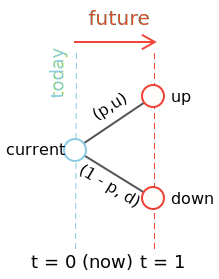
\includegraphics[width=0.30\textwidth]{./figs/Fig-OneStep-Binomial-Lattice-Schematic.pdf}
    \caption{Schematic of a single-period binomial lattice model. 
	In the future, the world can probabilistically move to the \texttt{up} state with probability $p$ or to the \texttt{down} state with probability $(1-p)$. 
	}\label{fig:example-oneste-binomial-lattice-schematic}
\end{figure}
The \texttt{up} and \texttt{down} factors $u$ and $d$, and the probability $p$ can be defined in various ways.  
Let's consider two approaches for computing the tuple $(u,d,p)$: real-world probabilities, which can be estimated from historical data, and risk-neutral probabilities, 
which are hypothetical probabilities that allow us to price assets as if investors are risk-neutral. 

\subsubsection{Estimating real-world probabilities}
We'll estimate values for $(u,d,p)$ lattice parameters by analyzing the reported interest rate data. 
Suppose the interest rates were continuously compounded such that:
\begin{equation}
r_{j} = r_{i-1}\cdot\exp\left(\mu_{j,j-1}\cdot\Delta{t}\right)
\end{equation}
where $r_{\star}$ denotes the rate at time index $\star$, $\mu_{j,j-1}$ denotes the annual growth rate of $r$ between time index 
$j-1\rightarrow{j}$, and $\Delta{t}$ denotes the time difference between time index $j - 1\rightarrow{j}$ (units: years). 
We can rearrange and estimate the growth rate values from the reported interest rate values:
\begin{equation}
\mu_{j,j-1} = \left(\frac{1}{\Delta{t}}\right)\cdot\log\left(\frac{r_{j}}{r_{i-1}}\right)
\end{equation}
for each time interval $j - 1\rightarrow{j}$ in the data. Assuming we have $N$ observations, we can estimate $N-1$ values for the 
growth rate $\mu$, from which we can estimate the \texttt{up} and \texttt{down} factors $u$ and $d$ using something like Algorithm \ref{algo-log-return-change-interest-rates}.

\begin{algorithm}[h]
    \caption{Logarithmic Growth Rate T-bill Yield}\label{algo-log-return-change-interest-rates}
    \begin{algorithmic}[1]

        \Statex
        \Require data set $\mathcal{D}_{i} = \left\{r_{i,t}\right\}_{t=1}^{N}\in\mathcal{D}$ where $r_{i,t}$ denotes the yield of T-bill with maturity $i$ at time $t$, 
		and $\mathcal{D}$ denotes the data set of all T-bills.
        \Require The time interval $\Delta{t}$ between $t$ and $t-1$ (units: years) and a list of maturities $\mathcal{L} = \left\{i\right\}_{i=1}^{M}$ for the T-bills in $\mathcal{D}$ where $M = \dim\mathcal{L}$.
		\Require All T-bills have the same number of trading days $N$.
     
        \Statex
		\Procedure{log growth rate}{$\mathcal{D}$, $\mathcal{L}$, $\Delta{t}$}
		\State{$N\leftarrow\text{length}(\mathcal{D})$}\Comment{Number of trading days for $i\in\mathcal{L}$}
        \For{$i\in\mathcal{L}$}
			\State{$\mathcal{D}_{i} \gets \mathcal{D}[i]$}\Comment{Select the data for maturity $i$ from the dataset $\mathcal{D}$}
            \For{$t=2\rightarrow{N}$}
                \State{$r_{i,t-1} \gets \mathcal{D}_{i}[t-1]$}\Comment{Select the price of stock $i$ at time $t-1$}
                \State{$r_{i,t} \gets \mathcal{D}_{i}[t]$}\Comment{Select the price of stock $i$ at time $t$}
                \State{$\mu^{(i)}_{t,t-1} \gets \left(1/\Delta{t}\right)\cdot\ln\left(r_{i,t}/{r_{i,t-1}}\right)$}
            \EndFor
        \EndFor
        \Statex
        \Return{$\mu^{(1)},\dots,\mu^{(\dim\mathcal{L})}$}\Comment{Return the logarithmic growth rate array for each T-bill $i\in\mathcal{L}$}
		\EndProcedure
    \end{algorithmic}
\end{algorithm}

\begin{concept}[Real-world Rate probabilities]\label{concept:real-world-interest-rate-probabilities}
We can estimate the real world probability $p$ by counting the number of times $\mu_{j,j-1}>0$ and 
dividing by the total number of observations. Similarly, we can estimate the \texttt{up} and \texttt{down} factors $u$ and $d$ 
by computing the average $\mu_{j,j-1}\cdot{\Delta{t}}$ when the rate increases or decreases, respectively.
\end{concept}
Then we can estimate the \texttt{up} and \texttt{down} factors $u$ and $d$ from the growth rate array 
generated using something like Algorithm \ref{algo-ud-estimation-rates}. 
\begin{algorithm}[h]
	\caption{Estimating $u$, $d$ and $p$ from the $\mu$-array}\label{algo-ud-estimation-rates}
	\begin{algorithmic}[1]

		\Require Growth-rate $\mu$-array from Algorithm \ref{algo-log-return-change-interest-rates}.
		\Require Effective risk-free rate $\bar{r}$ (units: inverse years).
		\Require time step size $\Delta{t}$ between $t$ and $t-1$ (units: years) of the price data
		\Require \texttt{mean} function, \texttt{find} function, \texttt{length} function, and \texttt{push} function.

		\Statex
		\Procedure{real world probability}{$\mu$, $\bar{r}$, $\Delta{t}$}
		\State
		\State{\textit{Initialize}:}
		\State{$N\leftarrow\text{length}(\mu)$}\Comment{Number of growth rates}
		\State{$\text{up}\leftarrow\text{Array}()$}\Comment{Initialize empty array of \texttt{up} factors}
		\State{$\text{down}\leftarrow\text{Array}()$}\Comment{Initialize empty array of \texttt{down} factors}
		
		\Statex
		\State \textit{Compute $u$:}
   	 	\State{$i_{+}\leftarrow \text{find}(\mu>0)$}\Comment{Find the indices of all \texttt{positive} growth rates}
    	\For{$i\in {i_{+}}$}
			\State{$\text{push}(\text{up}, \exp(\mu[i]\cdot{\Delta{t}})))$}\Comment{Push the \texttt{positive} return $\mu\cdot\Delta{t}$ onto $\text{up}$-array}
    	\EndFor
		\State{$u\leftarrow\text{\texttt{mean}}(\texttt{up})$}\Comment{mean is our estimate of the \texttt{up} factor $u$}
    	
		\Statex
		\State \textit{Compute $d$:}
   	 	\State{$i_{-}\leftarrow \text{find}(\mu<0)$}\Comment{Find the indices of all \texttt{negative} growth rates}
    	\For{$i\in {i_{-}}$}
			\State{$\text{push}(\text{down}, \exp(\mu[i]\cdot{\Delta{t}}))$}\Comment{Push the \texttt{negative} return $\mu\cdot\Delta{t}$ onto $\text{down}$-array}
    	\EndFor
		\State{$d\leftarrow\text{\texttt{mean}}(\texttt{down})$}\Comment{mean is our estimate of the \texttt{down} factor $d$}



		\Statex
		\State{$N_{+} \leftarrow\text{length}(i_{+})$}\Comment{Number of \texttt{positive} growth rates}
		\State{$p\leftarrow N_{+}/N$}\Comment{Estimate of the probability $p$}
		\Statex

		\State
		\Return{$u$, $d$ and $p$}
		\Statex
		\EndProcedure
	\end{algorithmic}
\end{algorithm}


\clearpage
\bibliography{References_v1}

\clearpage
\printindex

\end{document}
